\documentclass[a4paper,12pt]{article}

\usepackage[utf8]{inputenc}
\usepackage[ngerman]{babel}
\usepackage[T1]{fontenc}
\usepackage{graphicx}
\usepackage[cache=false]{minted}
\usepackage{dirtree}
\usepackage{biblatex}
\usepackage[strings]{underscore}
\addbibresource{literatur.bib}



\begin{document}
\begin{titlepage}
    \begin{center}
        \vspace*{1cm}
        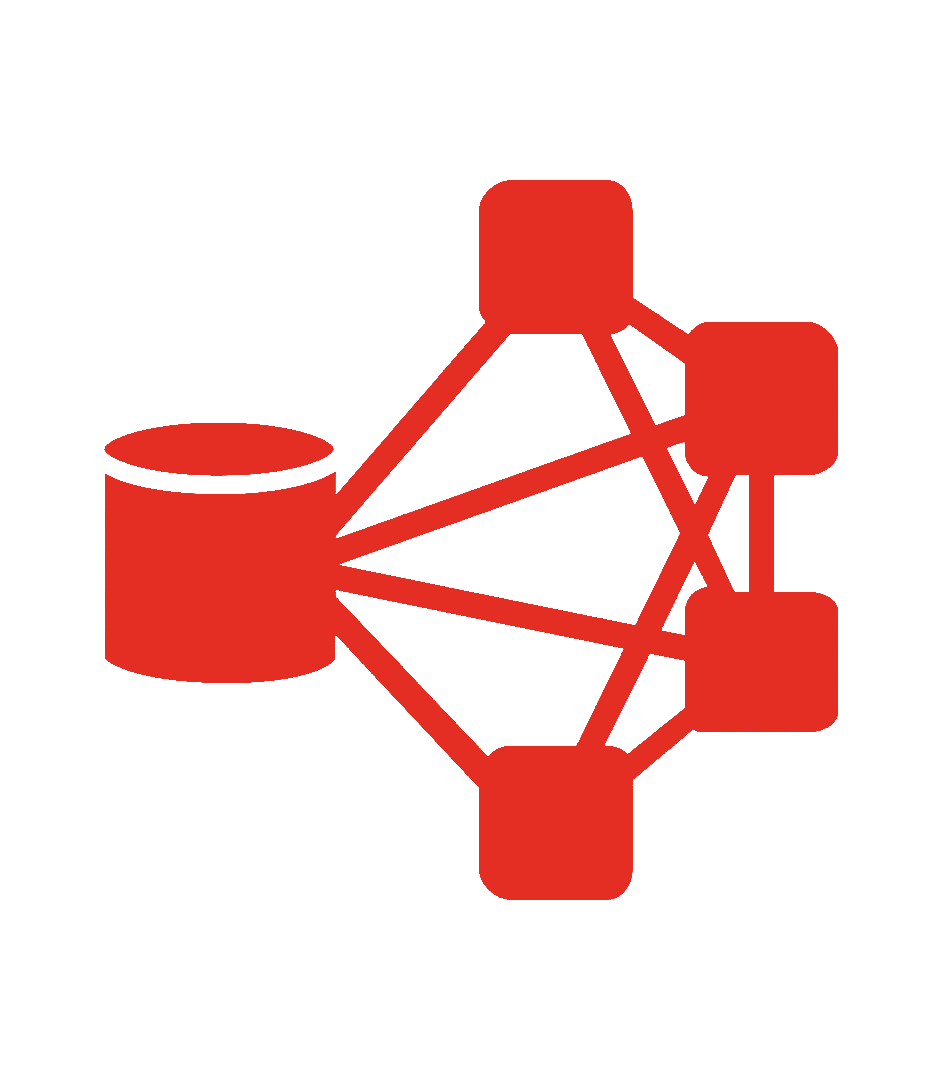
\includegraphics[width=10cm]{Logo.png}
        
        \textbf{\huge MapReduce-System}
        
        \vspace{0.5cm}
        NVS Projekt 2
                 
        \vspace{1.0cm}
    
        \textbf{Alexander Grill 5CHIF}
        
        \today
        
        \vfill
                 
                 
        \vspace{0.5cm}
                 
        Informatik\\
        HTBLUvA Wr.Neustadt\\
        Österreich\\

                 
    \end{center}
\end{titlepage}  
\newpage
\tableofcontents
\newpage


\section{Einführung}
In diesem Kapitel werden die Gründe der Umsetzung und das Thema, worum es in dieser Arbeit geht, genau erläuter. Es wird auch
darauf eingegangen, welche Thematiken das Projekt umfassen soll und wie sich die Benotung auseinandersetzt.

\subsection{Vorwort}
Der Virus "COVID-19" war im Jahr 2020 für die gesamte Bevölkerung auf der Erde eine riesengroße Herausforderung. Die Situation änderte sich am Begin des darauffolgenden Jahres 2021 nicht.
Deshalb beschloss die Bundesregierung weitere Maßnahmen, Ausgangsbeschränkungen, Grenzkontrollen, FFP2-Maskenpflicht und weitere Regeln einzuführen die die Bevölkerung einzuhalten hat. Alle Schüler in Österreich müssen die Schule 
blockweise besuchen. 
Nur mit einem davor verpflichtetenden Schnelltest und FFP2-Masken dürfen sie die Schule betreten. Da die Projektarbeiten im ersten Semster entsprechend gut ausgefallen sind, beschloss Herr Professor 
Kolousek, dass Schüler in den fünften Klassen im Fach NVS statt der Praktischen Arbeit und dem Theorietest eine Projektarbeit über den Semsterstoff machen müssen. Folgenddessen muss die Dokumentation über das gewählte Thema dementsprechend einen
weiteren Umfang umfassen, als beim ersten Projekt im ersten Semster. Im praktischen Teil geht es in diesem Projekt darum, ein Map-Reduce System in Kombination mit Server-Client Kommunikation zu implementieren. Im theoretischen Teil werden die Grundlagen, die für die 
Umsetzung relevant sind, erklärt. Zusätzlich beinhaltet dies auch sämtliche Abschnitte, wie die Source Code Dokumentation, Abläufe, Erklärung bezüglich MapReduce-System, Aufbau und Anwendungsfälle.
\begin{description}
    \item[Die zu erreichende Note hängt prinzipiell ab von der] ~\par
    \begin{itemize}
        \item Beispielkategorie
        \item Art der Kommunikation
        \item Funktion, Umfang und Tiefe der Implementierung
        \item Fehlerbehandlung
        \item Ausgaben, Einhaltung der Coding Conventions, Kommentare
        \item Repository: Commits, Issues
        \item Ausarbeitung
        \item Einhaltung der Richtlinien
      
    \end{itemize} 
\end{description}
\subsection{Motivation}
In diesem NVS Projekt geht es darum, ein MapReduce-System mit der Programmiersprache C++ unter Linux mittels g++ Compilier umzusetzten.
Kurz zusammengefasst soll eine große Menge an komplexen, unstrukturierten und eine Art von aufwendigen Daten verarbeitet werden. 
Das heißt, es sollen Daten, die planlos abgespeichert sind, zusammengefasst werden, sodass diese wieder ihren Nutzen oder Sinn erbringen. 
Diese können dann für weiter Verarbeitungsschritte oder Datenanalysen verwendet werden. Die Daten werden am Beginn in kleine 
Pakete aufgeteilt und diese werden mit einem eindeutigen
Schlüsse identifiziert. 
In der nächste Phase werden die einzelnen Pakete parallel von unterschiedlichen, getrennten und unabhängigen Prozessen 
zusammengefasst. Danach werden die gruppierten Daten wieder 
einem Schlüssel zugeordnet, sodass diese wieder zusammengefasst und minimiert werden. Die Kommunikation zwischen den einzelnen 
Knoten soll in dieser Arbeit mittel Server-Client Kommunikation passieren.
Der Server hört auch einen Port ab, ob sich ein Client damit verbinden möchte. Wenn eine Verbindung aufgebaut werden kann, soll die 
Splittung der Daten passier, daraufhin soll das Resultat weiter an den Server gegeben werden, bis 
alle Daten vereint auf dem Master Server liegen. Die bearbeiteten Daten werden schlussendlich in einem JSON-File abgespeichert.

\section{Aufgabenstellung}
Dieses Kapitel umfasst die genaue Erläuterung der Aufgabenstellung, sowie die Themenbereiche dieser Projektarbeit. Darüber hinaus wird auch über die Idee der Umsetzung geschrieben.
\subsection{Erläuterung der Aufgabenstellung}
Ziel ist es, dass eine Menge von unstrukturierten Daten so verarbeitet werden, dass diese danach wieder in ordnungsgemäßer 
Struktur vorliegen. Zuerst müssen die Daten aufgeteilt werden. Sie werden in einer Key-Value Form abgepeichert, somit kann
der Value, also der abgespeicherte Datensatz, mittels Key eindeutig identifiziert werden. Nachdem die Daten zusammengefasst vorliegen, 
werden sie im nächsten Schritt auf einzelne Knoten aufgeteilt. Diese erlangen von den einzelenen Clients die Daten in Key-Value Form und 
fassen diese wieder zusammen, bis die Daten zu einem Master Knoten ankommen und dort schlussendlich in geordneter Form darliegen.
Die Aktionen der Datenverarbeitung verlaufen ständig unter paralleler Abfolge. Die Aufgaben werden aufgeteilt und laufen auf 
verscheidenen Knoten.

\subsection{Idee}
Das Projekt ist so aufgebaut, dass es acht oder mehr Clients gibt, zwei Slave Server und einen Master Server. 
Ein Benutzer (Client) kann eine beliebige Anzahl von Zeichenketten, die er dem Programm beim Aufruf mitübergibt, 
erzeugen und diese werden dann in einer Datei abgespeichert. 
Zusätzlich wird dem Benutzer auch angeboten, den Speicherort der Datei selbst auszuwählen. 
Nachdem die ungeordneten Daten in einer Datei 
abspeichert sind, beginnt die nächste Phase des Map-Reduce Systems.
Die Datei wird zeilenweise durchgegangen. 
Die Zeichenketten werden in einem Art Dictionary als Key-Value Form abgespeichert, dadurch kann jeder eingefügte Datensatz identifiziert werden. 
Wenn der Datensatz in diesem Dictionary schon existiert, dann wird der Value, der als Counter festlegt, wie oft die Zeichenfolge im Text vorkommt, um eins erhöht. 
Nachdem kompletten Durchlauf der Datei sind alle Daten in diesem Dictionary abgespeichert. 
Dadurch, dass mehrere Clients das System zum gleichen Zeitpunkt unabhängig voneinander nutzen können, wird das Durchforsten der Datei von anderen Prozessen nicht beeinflusst. 
Nachdem ein Prozess mit der Datenabspeicherung fertig ist, sendet er die Daten an den jeweiligen Slave Server, der zu diesem Zeitpunkt nicht beschäftigt ist. 
Wenn der Server von einer gewissen Anzahl von Clients die Daten bekommt, beginnt er danach mit der Map Phase. 
An dieser Stelle werden die gesendetetn Daten wieder per Key zusammengefasst und strukturiert. 
Die Abarbeitung erfolgt auch in diesem Fall parallel zu einem weiteren Slave Knoten, der die selbe Art und Weise der Datenverarbeitung nutzt. 
Schlussendlich wird das Result an den Master Server geschickt. Jetzt bringt dieser all seine empfangenen Daten in eine Struktur, die im Nachhinein für Datenanalysen eingesetzt werden können.
\subsection{Themenbereiche}
\begin{description}
    \item[Diese Arbeit umfasst folgende Thematiken] ~\par
    \begin{itemize}
        \item Grundlagen und Basiskonzepte, Nachrichtenübertragung, Netzarchitektur
        \item Internetprotokoll
        \item Transportprotokolle
        \item Prozesse und Threads
        \item Synchronisation und parallele Programmierung
        \item Kommunikation, Serverprogrammierung, verteilte Systeme
        \item TCP/IP Programmierung      
    \end{itemize} 
\end{description}
\newpage
\section{Grundlagen}

\subsection{Was ist ein MapReduce System?}
Das Verfahren wurde 2004 von Google für die Indizierung von Webseiten entwickelt. 
Das Framework wird bei Datenbanken eingesetzt und dient zur Verarbeitung von großen, komplexen, unstrukturierten Datenmengen.
Dieses Verfahren findet Anwendung für BigData und Datawarehouse, weil in solchen Fällen 
große Datenmengen in kürzester Zeit mittels Software verarbeitet, analysiert, aggregiert als auch kompremiert werden. 
Map Reduce parallelisiert die Bearbeitung durch die Verteilung auf mehrere gleichzeitig auszuführende Tasks. 
Der Grund, warum dieses Framework solche Datenmengen verarbeiten kann ist, weil die Aufgaben auf mehrere Rechnern aufgeteilt werden. 
Jeder einzelne Rechner startet Prozesse, die parallel die Daten verarbeitet und auswertet.
Ein einzelner Rechner stößt schnell an seine Grenzen, deshalb ist die Verarbeitung von Daten mittels mehreren Knoten sehr effizient und bietet eine bessere Performance.
Das Verfahren wurde in vielen verschiedenen Verfahren eingesetzt, wie zum Beispiel für die Indizierung von Webseiten, 
nach einer Suchanfrage mit beliebigen Zeichenketten. Auch im Umfeld von Google News wird MapReduce verwendet. 
Andere große Internetfirmen wie Yahoo, die ebenfalls das Verfahren für die Indexierung von Webseiten verwenden, 
als auch Facebook verwendet das System, um Spam Messages zu minimieren und die Ads zu optimieren. 
Amazon hingegen verwendet das Verfahren für das Clustering der Produket. 
Ein Cluster ist eine Gruppe von Objekten mit ähnlichen Eigenschaften.
Im technischen Bereich werden Cluster dazu genutzt um Produkte, Einzelteile oder Baugruppen nach bestimmten Gesichtspunkten zu gruppieren.

\subsection{Map und Reduce}
Die beiden Grundfunktionen des Verfahrens sind Map und Reduce. 
Sie sorgen für die Aufteilung der Aufgaben in kleinere parallelisierte Arbeitspakete und führen am Ende die Ergebnisse zusammen. 
Bei großen relationalen Datenbanken und komplexen Queries lassen sich typische Probleme, bezüglich Verarbeitung von großen Datenmengen beseitigen.
Die Map Funktion verteilt die Aufgaben an unterschiedlichen Knoten eines Clusters. 
Die Reduce Funktion sortiert die verfassten Ergebnisse und fügt sie am Ende wieder zusammen.
Die Funktionen Map und Reduce werden vom User bereitgestellt, weil diese schließlich zu den bereitgestellten Daten passen müssen.
\cite{mrsystem}
\newpage

\subsection{Ablauf}

\begin{figure}[h]
    \centering
    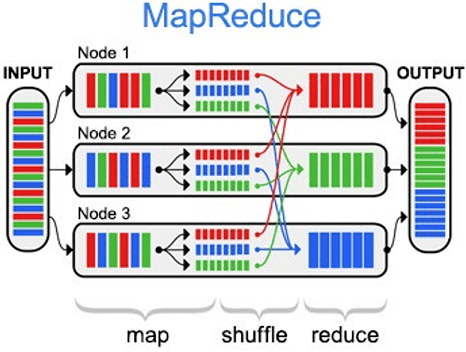
\includegraphics[width=6.1cm]{mapreduce.png}
    \cite{mrsystempic}
\end{figure}
\begin{description}
    \item[Das Verfahren verläuft durch folgende Schritte:] ~\par
    \begin{itemize}
        \item Split
        \begin{itemize}
            \item{Die bereitgestellten Daten werden aufgeteilt. Jeder Datensatz darin ist durch
            einen Schlüssel-Wert identifiziert. Diese Datenmenge wird nun in kleinere Datenmengen aufgeteilt
            und vom Master an die verfügbaren Knoten verteilt.}
        \end{itemize}
        \item Map 
        \begin{itemize}
            \item{Nun wendet jeder Knoten auf die Daten die Map-Funktion an, die schließlich Key/Value Paare zurückgibt. Diese Ergebnisse werden zwischengespeichert.}
        \end{itemize}
        \item Shuffle
        \begin{itemize}
            \item{Bei diesem Schritt geht es darumm denn reduce-Knoten die entsprechenden Daten zuzuteilen.
            Diese Zuteilung entspricht einer Fragmentierung.
            Hierbei wird dem Knoten, die reduce ausführen, ein Key zugeteilt. Diese Knoten holen sich
            dann die bereits durch Map entstandenen Datensätze mit diesem Key und wenden reduce an.}
        \end{itemize}
        \item Reduce
        \begin{itemize}
            \item{Grundsätzlich ist die Aufgabe dieser Funktion die Key/Value Paare anhand des Schlüssels
            zusammenzufassen und dabei die Summe der einzelnen Values zu bilden. Demnach ist die
            Ausgabe der Reduce-Funktion wieder ein Key/Value Paar mit dem gleichen Aufbau wie vor
            der Verarbeitung.
            Dies ermöglicht es, dass reduce mehrere Male angewendet werden kann, bis schließlich alle
            Daten gesammelt wurden.}
        \end{itemize}
    \end{itemize} 
\end{description}

\subsection{Vorteile und Nachteile eines Map-Reduce Systems}
Map Reduce bietet eine Menge an Vorteilen gegenüber dem klassischen Verfahren der Datenverarbeitung, wie
sie in den relationalen Datenbanksystemen verwendet werden. \\ \\
Ein wesentlicher Vorteil ist, dass für die
Verwendung eines solchen System ein einfacher normaler Rechner benötigt wird und keine Highend-Server. Ein Cluster-Verbund für die parallelisierte
Datenverarbeitung kann bei Notwendigkeit ohne großen Aufwand realisiert werden. Ein Cluster-Verbund ist ein Netzwerk, das aus mehreren Rechner besteht, die gleichzeitig miteinander verbunden sind 
und Daten austauschen. Aus diesem Grund ist ein MapReduces-System sehr kostensparend und kann mit wenig Know-How und Erfahrungen umgesetzt und
schlussendlich in Verwendung gebracht werden. \\ \\
Ein weiterer Vorteil ist auch die Skalierbarkeit. Da die Daten auf den jeweiligen Knoten
aufgeteilt werden, bietet das System eine zuverlässige Ausfallstoleranz und Verfügbarkeit, denn wenn ein Knoten ausfallen sollte, werden die Daten einfach an einen
anderen Knoten weitergeleitet und dort verarbeitet, somit läuft das System jederzeit in einem stabilen Zustand. \\ \\
Durch die parallelisierte Verarbeitung von Daten ist dieses Verfahren deutlich effizienter und perfomanter als die Datenverarbeitung
in relationalen Datenbanken. Im Terabyte-Bereich dauert das Verfahren oft nur Minuten, im Petabyte-Bereich Stunden, wobei andere Systeme deutlich mehr Zeit und Ressourcen für die Verarbeitung
benötigen.\\ \\
Während die Berechnungen schnell gehen, dauert der Datenzugriff länger als bei anderen Methoden. 
Die Daten müssen erst über das Netzwerk gestreamt werden. Dabei ist die Netzanbindung der Flaschenhals, vor allem im Hinblick auf die sehr unterschiedlichen Rechner innerhalb des Clusters und deren unterschiedliche schnelle Netzanbindung.\\ \\
Um die Geschwindigkeit zu erhöhen, kann ein Cluster ausschließlich aus High-End-Servern bestehen. In diesem Fall sind die Kosten für das MapReduce-Verfahren immens hoch.
\cite{vorteil/nachteilemrsystem}
\newpage
\noindent
\subsection{Parallel Programming}
Unter Parallel Programming versteht man die Aufteilung einer Problemstellung in weitere kleinere Teilprobleme, die nebenläufig abgearbeitet werden. Dabei wird jedes Teilproblem einzeln gelöst und dadurch kann auch das Gesamtproblem effizient und schnell gelöst werden. 
\\Gleichzeitig kann die Problemstellung schneller gelöst werden, weil die Abarbeitung aufgeteilt wird und die Teilprobleme unabhängig voneinander gleichzeitig bearbeitet werden können. Parallel Programming wird heutezutage in Branchen wie Chemie, Biologie, Medizin, Maschinenbau, Baustatik, Simulationen, Suchen in großen Datenbestände etc. angewendet.\\\\
\textbf{Mooresches Gesetz\\}
"Die Anzahl der Transistoren pro Chip verdoppelt sich etwa alle zwei Jahre". Das heißt, je mehr Transistoren sich auf einem Chip befinden, desto mehr Funktionalität kann parallel abgearbeitet werden. Laut der Webseite "nature.com" wird die Halbleiterindustrie im März 2016 anerkennen, dass Moore's Law nicht mehr eingehalten werden kann. Demnach werden Chips nicht mehr zwangsläufig schneller, aber Fortschritt und Effizienzmaximierung wird es weiterhin geben.\\\\
\textbf{Wirth´sches Gesetz\\}
"Die Software wird schneller langsamer, als die Hardware schneller", darunter versteht man, dass die Anforderungen an die Software immer aufwendiger, größer und komplexer wird und die Hardware diese Softwaren sehr langsam bis gar nicht verarbeiten können.\\\\
\textbf{Taktfrequenzen\\}
Die Taktfrequenze verdoppelte sich in den 1990-er Jahre alle 18 bis 20 Monate, aber seit 2000 bis 2005 ist das nicht mehr der Fall. Heute finden maximial 4GHz im Desktop und Serverbereich Anwendung.\\Man spricht von einer sogenannten "Frequency Wall", wenn die Taktfrequenz nicht mehr erhöht werden kann, weil höhere Frequenz höhere Spannung bedeutet, höhere Spannung heißt, höhere Verlustleistung. Das hat zur Folge, dass die entstehende Wärme, die durch den Anhieb der Taktfrequenz und durch die Datenverarbeitung entsteht, nicht mehr abgeführt werden kann.
Existierende nicht parallelisierte Software profitiert nicht mehr automatisch von der Leistungssteigerung der Hardware. Ein weiterer Nachteil ist, dass das Laufzeitverhalten paralleler Algorithmen schwieriger nachvollziehbar sein kann, als das eines äquivalenten sequentiellen Algorithmus.\\\\
\textbf{Lösungsansätze\\}
Der einfachste Lösungsansatz ist der, indem man den Problemraum einschränkt. Damit ist gemeint, der Algorithmus wird für den jeweiligen Aufwand eingeschränkt und angepasst. Eine weitere Idee wäre, dass man den Algorithmus selbst optimiert, jedoch ist das nicht immer möglich. Weiters ist die Verbesserung der Implementierung von Vorteil. (z.B Facebook -> eigener String)
Auch durch den Bereich Hardware kann eine Software verbessert werden, dennoch ist diese Strategie mit hohen Kosten verbunden. Am effizientesten ist es hingegen, die Software in Teilprobleme aufzuteilen und diese parallel abzuarbeiten. Da ein Prozessor mehrere Kerne besitzt, können mehrere unterschiedliche, unabhängig voneinander, Prozesse abgearbeitet werden. 
\begin{description}
    \item[Möglichkeiten der Parallelisierung] ~\par
    \begin{itemize}
        \item Zerlegung der Gesamtaufgabe in kleinere, mehrere Teilaufgaben, sodass die maximale Auslastung aller Prozesser(HW) stattfindet, weil jede Teilaufgabe auf einem einzelnen Prozessor stattfindet.
        \item Zerlegung der Gesamtaufgabe in kleinere, mehrere Teilaufgaben, die hintereinander ausgeführt werden, allerding wird die Gesamtzeit der Lösung einer Gesamtaufgabe nich kürzer und der Durchsatz bei der Lösung von vielen Aufgaben höher.
        \item Zerlegung der Gesamtaufgabe in kleinere, mehrere Teilaufgaben, die hintereinander ausgeführt werden, aber mit spezieller Hardware gelöst werden.
    \end{itemize} 
\end{description}
\textbf{Pipelinig\\}
Pipelinig beschreibt den Vorgang wie ein Prozessor vorgeht, wenn er mehrere Befehle verarbeiten muss. Als Erstens wird der Befehl aus dem Arbeitsspeicher geladen(fetch), weiters wird dieser Befehl in Maschinensprache umgewandelt und dekodiert(decode). Werden zusätzliche Daten benötigt, lädt der Prozessor diese aus Registern oder aus dem Arbeitspeicher. Folgedessen wird der Befehl ausgeführt(execute) und das Resultat des Befehls wird in einem Register oder im Arbeitspeicher geschrieben (write back).
Die einzelnen Schritte werden in einer eigenen Hardwarekomponente ausgeführt, deshalb ist es möglich, wenn ein Befehl gefetched wird und danach dekodiert werden kann, kann in der Zeit, in der er dekodiert wird, ein andere Befehl gefetched werden, weil die Hardwarekomponente nicht verwendet wird. Das ist bei jedem einzelnen Schritt beim Pipelinig möglich. Die Abarbeitungzeit der einzelnen Prozesse wird nicht minimiert, hingegen können mehrere Prozesse in einer Zeitspanne abgewickelt werden, d.h. der Durchsatz ist höher.\\
\textbf{Probleme\\}
Befehle, zwischen denen Abhängigkeiten herrschen, können zu Problemen führen. Dabei kann es zu einer längeren Abarbeitung der Prozesse kommen, weil einzelne Prozesse auf das Ergbniss des davor durchgeführten Prozesses warten.\\ Zusätzlich kann zwischen den Prozessen nicht nur eine Datenabhänigkeit herrschen, sonder auch eine Abhängigkeit im Kontrollfluss. In diesem Fall existiert eine Abhängigkeit zwischen den Prozessschritten selbst. Wie in der Datenabhänigkeit müssen auch hier Wartezyklen eingeführt werden.\\
Weiters kann auch passieren, dass die Abarbeitungsschritte vom Prozessor selbst umgeordnet werden, obwohl es zwischen den Anweisungen Abhängigkeiten herrschen. Diese werden vom Prozessor nicht berücksichtigt.\\
Daten, die für einen Prozess benötigt werden, können schon weit vor der Benutzung aus dem Hauptspeicher gelesen werden und schlussendlich auch für die Abarbeitung verwendet werden. Hier kann es zu Problemen kommen, wenn nicht aktuelle Daten oder falsche Daten gelesen werden, weil das Result nicht den gewünschten Wert hat.\\\\
\textbf{Superskalarität\\}
Superskalare Prozesse enthalten mehrere gleichartige Funktionseinheiten, zum Beispiel Rechenwerke für Ganzzahl- und Gleitkommaarithmetik oder Lade- und Speichereinheiten. Damit können mehrere Befehle parallel ausgeführt werden, wenn keine Abhängigkeiten existieren.\\\\
\textbf{Hardware seitiges Multithreading\\}
Wenn mehrere Threads auf ein Szenario warten, können daher in der Zwischenzeit Befehle eines anderen Threads durchgeführt werden, dazu werden aber mehrere Registersätze benötigt.
Die Hardwarethreads erscheinen dem Benutzer wie echte Kerne des Prozessors, obwohl sie keine sind. Der Performancegewinn liegt bei ca 10 bis 20\%.\\\\
\textbf{Vectoreinheiten\\}
Um die Abarbeitung zu beschleunigen, können sogenannte Vectoreinheiten eingesetzt werden, dabei kann ein Befehl mehrere Daten zur selben Zeit verarbeiten.\\
Parallele Architekturen lassen sich auf unterschiedliche Arten klassifizieren. Eine sehr grundlegende Einteilung von Computersystemen allgemein stellt „Flynn’s Taxonomy“ dar. Diese behandelt nicht allein parallele Systeme, beinhaltet diese aber, was verdeutlicht, dass Parallelisierung bereits vor über 40 Jahren ein Thema war.
\newpage
\noindent
Eine mögliche Kategorisierung von ausschließlich parallelen Systemen kann nach der Art der Speicherverwaltung getroffen werden.
Unabhängig davon, welche Klassifizierung herangezogen wird, ist jedoch zu erwähnen, dass die Übergänge zwischen den Kategorien oft fließend sind. Viele Lösungen sind also durchaus in unterschiedliche Bereichen einzuordnen.
\begin{description}
    \item[Flynnsche Klassifikation] ~\par
    \begin{itemize}
        \item SISD single instruction, single data
        \begin{itemize}
            \item{klassische Von‑Neumann Architektur}
        \end{itemize}
        \item SIMD single instruction, multiple data
        \begin{itemize}
            \item{Vektorprozessoren}
        \end{itemize}
        \item MISD multiple instructions, single data
        \begin{itemize}
            \item{theoretischer Natur}
        \end{itemize}
        \item MIMD multiple instructions, multiple data
        \begin{itemize}
            \item{Multicore‑ und Multiprozessorsysteme\\\\}
        \end{itemize}
    \end{itemize} 
\end{description}
\textbf{Rechnerarchitekt\\}
Man unterscheidet zwischen einem homogenen und einem heterogenen Aufbau. Beim homognenen Aufbau haben alle Rechner die gleichen Hardwarekomponenten und beim heterogenen Aufbau haben die Rechner verschiedenartige Prozessoren, Kerne usw.\\
Bei der Speicherarchitektur gibt es ebenfalls zwei unterschiedlich Arten, nämlich UMA (uniform memory access) und NUMA(none uniform memory access). Bei der UMA Variante haben alle Prozessoren und Kerne Zugriff auf den gleichen Hauptspeicher. Bei der NUMA Variante, besitz jeder Prozess einen eigenen Speicher und der Zugriff auf einen Fremndenspeicher erfolgt über ein Verbindungsnetzwerk.\\
In der Rechnerarchitektur gibt es Multicore und Multiprozessor. Multi-Core bedeutet, dass in einem Prozessor mehrere Prozessor-Kerne eingebaut sind. Man bezeichnet diese Prozessoren als Multi-Core- oder Mehrkern-Prozessoren. Rein äußerlich unterscheiden sich Multi-Core-CPUs nicht von Single-Core-CPUs. Der Rechenkern ist bei Multi-Core-CPUs einfach mehrfach vorhanden. Innerhalb des Betriebssystems wird der Multi-Core-Prozessor wie mehrere Recheneinheiten behandelt.\\
\newpage
\noindent
\textbf{Parallelität in der Software\\}
Im Zeitalter exponentiell ansteigenden Datenverkehrs wird der Bedarf an harten und weichen Rechenkapazitäten immer größer. Auch die Rechenprozesse selbst werden deutlich komplexer und erfordern mehr Ressourcen. Eine Antwort darauf ist die Cloud, die der Nachfrage nach Serverleistung mit virtuellen Hostingdiensten nachkommt und so erheblichen Druck von Rechenzentren und Serverlandschaften nimmt.
Eine andere Antwort darauf sind Computer, die statt mit nur einem gleich mit mehreren Prozessorkernen ausgestattet werden. Damit schaffen sie ideale Bedingungen für die parallele Programmierung, weil sie eine nebenläufige, sprich parallele, Abwicklung mehrerer Rechenprozesse ermöglichen – so genannte Threads. Dabei spielt es keine Rolle, ob die Teilprozesse auf die Sekunde genau parallel verlaufen – vielmehr geht es darum, dass die Software dadurch verschiedene Dinge gleichzeitig erledigen kann, also die Fähigkeit zum Multitasking besitzt.\\\\
\textbf{Das Amdahl‘sche Gesetz\\}
Das Amdahl’sche Gesetz bezeichnet in der Informatik ein Modell zur Beschleunigung von Programmen durch Parallelisierung, deren Voraussetzung bekanntlich die Verwendung mehrerer Prozessoren ist. Verwendet man zum Beispiel doppelt so viele Prozessoren, benötigt man nach Amdahl im besten Fall die halbe Zeit zur Durchführung des Programms aka zur Lösung des Problems. Dabei wird die Temposteigerung allerdings dadurch ausgebremst, dass Programme niemals vollständig parallel operieren können und dass es immer einen gewissen Anteil an sequentiellen Programmteilen geben muss – etwa bei der Initialisierung oder in der Speicherverwaltung, weil diese Dinge entweder auf nur einem Prozessor ablaufen oder in Abhängigkeit zu anderen Ereignissen stehen. Deshalb sieht Amdahl vor, den Programmcode in sortenreine Abschnitte aufzuteilen – solche, die rein sequentiell und solche, die rein parallel operieren. Die komplette Dauer eines Programmes ergibt sich dann aus der Formel Z =zs +zp.
Amdahl beobachtet, dass bei steigender Anzahl der Prozessoren dieser Beschleunigungsfaktor (Speed-up) immer stärker von den sequenziellen Anteilen des Prozesses gehemmt wird, da mit der Inbetriebnahme weiterer Prozessoren auch weitere Aufwände anfallen, für die Initialisierung etwa oder für die Synchronisierung, sprich z0.
\cite{parallelprogramming}
\newpage
\noindent
\subsection{Kommunikation}
Das Prinzip der Kommunikation im Internet ist, dass man strikt sein soll beim Senden der Daten und tolerant beim Empfangen. Der Zweck einer Kommunikation ist die Interoperabilität, das bedeutet, 
dass mehrere Systeme, die aus Rechner bestehen, in der Lage sind, Daten untereinander auszutauschen. Die Fehlertolaranz bedeutet, dass die Daten durch festgelegte Regeln übertragen werden aber beim Empfangen in einer
gewünschten Form umgewandelt werden können.

\begin{description}
    \item[Beziehungen zwischen den einzelnen Knoten] ~\par
    \begin{itemize}
        \item one-to-one
        \begin{itemize}
            \item{Ein Knote kommuniziert mit einenm anderen Knoten}
        \end{itemize}
        \item one-to-many
        \begin{itemize}
            \item{Ein Knoten spricht mit mehreren Knoten und alle lauschen und hören zu. Diese Art von Kommunikation zwischen den Rechnern nennt man multicast}
        \end{itemize}
        \item one-to-any
        \begin{itemize}
            \item{Ein Knoten spricht mit mehreren Knoten, jedoch betrifft das nur einen Knoten von mehreren.}
        \end{itemize}
        \item many-to-one
        \begin{itemize}
            \item{Mehrere Knoten sprechen zu einem konkreten Knoten}
        \end{itemize}
        \item many-to-many
        \begin{itemize}
            \item{Mehrere Knoten kommunizieren mit mehreren anderen Knoten.\\}
        \end{itemize}
    \end{itemize} 
\end{description}
\textbf{Kommunikationsrichtung\\}
Beim Datenautausch ist wichtig festzuhalten, in welche Richtung die Daten übertragen werden. Mittels simplex werden die Daten nur in eine Richtung übertragen. 
Bei half-duplex werden die Daten ebenso in eine Richtung übertragen, jedoch kann die Richtung in der Übertragung geändert werden. Bei der Variante duplex werden die Daten in beide Richtungen übertragen. Wie im TCP Protokoll realisiert, werden zwei Streams
zur Verfügung gestellt, um Daten zu senden und zu empfangen.
\newpage
\noindent
\textbf{Verbindungen\\}
Im Grunde genommen unterscheidet man zwischen verbindungsorientiertern und verbindungsloser Kommunikation. Bei der verbindungsorientierter Kommunikation wird eine Verbindung zwischen zwei Knoten aufgebaut, danach werden Daten ausgetauscht und zum Schluss kommt es zum
Verbindungsabbau. Hingegen werden bei der verbindungslosen Kommunikation nur die Datenübertragen und keine Verbindung aufgebaut und abgebaut. Es ist in der Regel effizienter, aber es wird nicht sichergestellt, ob die Daten wirklich beim Empfänger angekommen sind.\\ \\
\textbf{Signalisierung\\}
Bei der Kommunikation werden auch Nachrichten ausgetauscht, die zum Aufbau, der Überwachung und dem Abbau einer Verbindung notwendig sind. Man spricht von in-bank signalling. Es wird ein gleicher logischer Kanal wie Nutzdaten und Steuerungsdaten verwendet, oder out-of-band signalling, hier wird ein getrennter logischer Kanal verwendet. Es gibt einen
physischen Kanal, der in mehrere logische Kanäle unterteilt ist. \\ \\
\textbf{Protokoll\\}
Für die Kommunikation benötigt man auch festgelegte Regeln, die für eine Kommunikation notwendig sind, darunter versteht man den Begriff Protokoll. Das betrifft das Format der Nachrichten, Reihenfolge der Nachrichten und die Spezifikation der Fehlersituation. Es gibt zustandsbehaftete und zustandslose Protokolle. Zustandsbehaftete Protokolle sind jene, bei denen die Nachrichten
vom Zustand der zuvor gesendete Nachrichten abhängt. Bei zustandlosen Protokol sind, die Nachrichten unabhängig von zuvor gesendeten Nachrichten.\\\\
\textbf{Session\\}
Im Informationaustausch spielt auch der Begriff Session eine wichtige Rolle. Dieser beschreibt eine feste Beziehung zwischen kommunizierenden Prozessen mit vereinbarten Eigenschaften, wie Namen, Ressourcen, Charakteristika. Dadurch bildet sich ein gemeinsamer Zustand zwischen den einzelnen Prozessen. Um sicherzustellen, welcher Knoten welcher ist und welche Rechte dieser
bei der Kommunikation mit anderen hat, werden Mechanismen zu Authentifikation und Autorisierung eingesetzt. Bei HTTP sieht die Kommunikation folgendermaßen aus. Ein Client der mittels Browser eine Seite aufruft sendet einen Request an den Server. Dieser überprüft die Daten der Anfragen und welche Daten der Client benötigt und sendet den Client danach mittels Respones die angefragten Daten zurück.\\
Wird die Seite neu geladen, so verschwinden auch die Daten, die in einem Cache zwischengespeichert sind und für weitere Aktionen relevant sind. Dies kann oft zu Problemen führen. Deshalb wird ein sogenanter Session-Cookie verwendet, in dem Daten abgelegt werden, die in einer Session entstehen und für weitere Tätigkeiten relevant sind und in diesem abgespeichert werden.\\ \\
\textbf{Hierachie von Protokollen\\}
Protokolle sind hierachisch angeordnet, das hat den Vorteil, dass man mit Problemen zwischen den unterschiedlichen Protokollen besser umgehen kann und jede Schicht nur wissen muss, was mit der darunterliegenden Schicht zu tun ist und wie man Daten an die darüberliegenden Schicht geben kann. Die Schichten können auch ausgetauscht werden.
\\\\
\textbf{Kommunikationsstile\\}
Die Kommunikation kann durch unterschiedliche Stilen durchgeführt werden. Zum Beispiel wird ein gemeinsamer genutzter Knoten verwendet und auf diesen zugegriffen, auf dem alle Daten abgespeichert werden, wie es bei Datenbanken der Fall ist. Beim Versenden von Nachrichten spricht man von nachrichten-orientierter Kommunikation.\\\\
Im Vergleich beim Aufruf einer Funktion oder Methoden, die auf einem Client abgespeichert sind,
spricht man von entfernter Funktionsaufrufe (entfernte Methodenaufrufe), wenn Daten verarbeitet werden oder wenn sie eintreffen, spricht man von stream-orientierter Kommunikation.\\\\
\textbf{synchron vs. asynchron\\}
Ein Nachrichtenautausch kann entweder synchron oder asynchron passieren. Bei einem synchronen Austausch wird die Operation begonnen, wenn der Sender die Nachricht initiert hat und der Empfänger bereit, ist die Nachricht zu empfangen. Bei einem asynchronen Nachrichtenaustauch ist es unabhängig davon, ob der Sender bereit ist oder nicht. 
\newpage
\begin{description}
    \item[Semantik der Nachrichtenübermittlung] ~\par
    \begin{itemize}
        \item no-wait-send
        \begin{itemize}
            \item{Der Sendeprozess wartet lediglich, bis die Nachricht im Transportsystem zum Absenden bereitgestellt ist.}
        \end{itemize}
        \item synchronization send
        \begin{itemize}
            \item{Der Sendeprozess wartet, bis die Nachricht vom Empfangsprozess entgegengenommen worden ist.}
        \end{itemize}
        \item remote-invocation send
        \begin{itemize}
            \item{Der Sendeprozess wartet, bis die Nachricht vom Empfangsprozess verarbeitet und beantwortet worden ist.\\\\\\}
        \end{itemize}
    \end{itemize} 
\end{description}
\textbf{transient vs. persistent\\}
Die Datenübertragen in einem Netzwerk kann transient sein (Message Passing), das heißt, beide Kommunikationspartner müssen online sein, weil das Kommunikationssystem Nachrichten nur solange speichert, wie die
sendende und die empfangene Operation ausgeführt wird. Unter Persistent (Message Queueing), versteht man, dass Kommunikationssystem Nachrichten speichert bis diese vollständig an den Empfänger ausgeliefert wurden.\\\\
Musterlösungen einer Datenübertragung kann request/response(A sendet an B, B sendet an A) sein, oneway(A sendet an B, A sendet an B), batching(Zusammenfassung von oneway Nachrichten) und publish/subscribe. Daten können durch zwei verschiedene Möglichkeiten interoperable übertragen werden, nämlich Daten werden ganz einfach in ein maschinenunabhängiges Format transformiert, oder der Empfänger muss sich um eine notwendige Konvertierung kümmern.\\ Im ersten Fall müssen beide Kommunikationspartner
die Daten so umwandeln, sodass diese für sie verständlich sind und im zweiten Fall spezifiziert der Sender den Datentyp aus einer Liste von vorgegebenen Datentypen.
\cite{communication1}
\newpage
\noindent
\textbf{Message Oriented Middleware\\}
Message Oriented Middleware ist eine Softwareinfrastruktur, die durch asynchrone Verbindung (nicht im klassischen Sinne, sondern im Sinne von Kommunikationsbeziehungen) charakterisiert ist und die sich mittels mehreren Systeme durch Nachrichten miteinander verbindet. Protokolle für MOM wären zum Beispiel: 
AMQP, STOMP, OpenWire, Java Message Service, XMPP, REDIS und MQTT.\\\\Im Unterricht wurde besonders auf das Protokoll MQTT Rücksicht genommen, weil es aktuell ist. MQTT ist ein Protokoll das ursprünglich von IBM zur Überwachung von Ölpipelines. Das Protokoll ist sehr leichtgewichtig gehalten, weil eine große Datenmenge
mittels einfachem Protokoll übertragen werden soll. \\\\
Das Protokoll basiert auf einem publish/subscribe Ansatz und die Idee dieses Protokolls ist, dass es kompatible mit anderen Programmiersprachen, wie C++, Java, .Net, Python, PHP usw. ist. Der Aufbau des Protokolls ist hierarchisch, wie unter Linux der Verzeichnisbaum. \\\\Der Vorteil ist der, dass man durch den hierarchisch Topic Aufbau, nur die 
Daten erhält, die man auch zwingend anfordert, Z.B bei etage1/wohnzimmer/ bekommt man nur alle Daten vom Wohnzimmer aus der ersten Etage und wenn man alle Daten von der ersten Etage möchte, fordert man mittels /etage1/ diese an. Wichtige Charakteristika sind auch Themen, wie Quaility of Service, Last Will and Testament, Retained Message und Authentifizierung.\\
\\
\textbf{Entfernte Funktionsaufrufe}\\
Unter Remote Procedure Call (RPC) versteht man, dass nach dem Funktionsaufruf der Prozess, der durch den Aufruf gestartet wird, auf einem anderem Host im lokalen Netzwerk gestartet wird. Die Zugriffstransparenz kann bei nachrichtenorientierter Kommunikation nicht erfüllt werden, wenn lediglicht eine Operation am Server ausgeführt werden soll. Dieses Konzept findet Anwendung auf Basis von Proxy-Pattern.\\\\
\newpage
\noindent
\textbf{Proxy-Pattern}\\
Elemente des Proxy-Patterns sind: Client-Objekt, Client Stub(Proxy), Server Stub(Sekeleton), Server-Objekt\\
\begin{figure}[h]
    \centering
    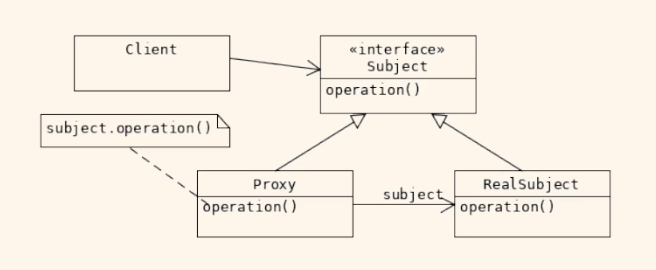
\includegraphics[width=8cm]{ProxyPattern.png}
\end{figure}
\\
Die Vorgehensweise sieht folgendermaßen aus: Ein User möchte auf einem Objekt eine Methode aufrufen er ruft die Methode nicht direkt auf dem Objekt auf, sondern der Client verwendet ein Interface. Die Implementierung des Interface kann entweder eine abstrakte Klasse sein oder
ein Interface, das vorgibt, welche Methoden definiert werden sollen bzw. zur Verfügung stehen.
Zusätzlich gibt es noch eine Klasse Proxy und RealSubject, auf dem die Operation die von oben vererbt wird, ausgeführt wird. Im Remote Proxy Pattern ruft ein Client mit dem Interface auf dem Proxy Objekt einer Operation auf. Diese Proxy Objekt dient als Stellvertretung des realen Objekts. Das Proxy Objekt baut nach der Ausführung der Operation
eine Verbindung zu dem wirklichen Objekt auf und über diese Verbindung wird ein Protokoll abgewickelt. Bei der Übertragung werden sämtliche Informationen bezüglich des Funktionsaufrufe wie zum Beispiel Eingangsparameter, Ausgabeparameter oder Funktionsname mit übertragen. \\\\
Nach der Ausführung wird das Resultat des Objekts anhand des Protokolls zurück zum Proxy Objekt und dann zum Client zurückgesendet. Der Aufruf wirkt wie ein lokaler Aufruf, jedoch funktioniert dies über das verwendete Netzwerk.
Das Sekeleton ist zuständig, die Kommunikation zwischen dem Proxy und dem RealSubject abzuwickeln.\\\\
Probleme, die bei der Umsetzung eines Proxy-Patterns auftreteb könnten sind vor allem Interoperabilitätsprobleme (Probleme die beim Zusammenspiel zwischen verschiedener Systeme, Techniken oder Organisationen auftreten), call-by-refernce, Behandlung von Excpetions, die Transparenz kann nicht gewährleistet werden und die Behandlung von Threads und Prozessen erfolgt nur serverseitig, Client findet den Server nicht, Client stürzt nach dem senden der Nachricht ab, Nachricht geht verloren, Server stürzt ab, Antwort geht verloren, Client stürzt ab, bevor diese die Antwort bekommt.
\newpage
\noindent
\begin{description}
    \item[Aufrufvarianten] ~\par
    \begin{itemize}
        \item synchrone Funktionsaufrufe: remote‑invocation send
        \item synchrone Prozeduraufrufe: synchronization send
        \item asynchrone Funktionsaufrufe: no‑wait send
        \item asynchrone Prozeduraufrufe: no‑wait send\\\\
    \end{itemize} 
\end{description}
\textbf{Stream-orientierte Kommunikation}\\
Stream-orientiert Kommunikation bezeichnet die gleichzeitige Übertragung und Wiedergabe von Video- und Audiodaten über ein Netzwerk.
Dabei werden Streams von Daten versendet, keine Nachrichten, sondern nicht abgeschlossene Informationeneinheiten.
Den Vorgang der Datenübertragung selbst nennt man Streaming und übertragene Programme werden als Livestream oder kurz Stream bezeichnet. Streaming-Media, das über das WWW bzw. HTML angestoßen wurde, wird auch Webradio oder Web-TV genannt. Im Gegensatz zum Herunterladen ist das Ziel beim Streaming nicht, eine Kopie der Medien beim Nutzer anzulegen, sondern die Medien direkt auszugeben, anschließend werden die Daten verworfen.
\\\\
Die Wiedergabe von Programmen über einen Livestream unterscheidet sich meist vom klassischen Rundfunk. Während beim Rundfunk an eine unbestimmte Anzahl Empfänger zugleich gesendet wird, handelt es sich beim Streaming meist jeweils um eine Direktverbindung zwischen dem Server des Senders und dem Client jedes einzelnen Benutzers. Die Verbreitung erfolgt oftmals über Streaming-Portale und internetbasierte Mediatheken.
\cite{communication2}
\newpage
\noindent
\subsection{TCP/IP}
Das Transmissioncontrollprotokoll und Internet Protokoll ist eine Menge von Kommunikationsprotokollen, die für den Verbindungsaufbau zu einem Netzwerk verwendet werden. TCP/IP kann auch als Kommunikation in einem Intranet(Firmen internes Internet) oder Extranet(betriebsinternes Computersystem, das für bestimmte externe Benutzergruppen geöffnet ist) eingesetzt werden.TCP/IP ist eine Reihe von Regeln und Verfahren wie der Datenaustausch abgehalten werden soll, dabei sind TCP/IP die Hauptprotokolle. TCP/IP definiert, wie Daten über das Internet übertragen werden, indem eine Ende zu Ende Kommunikation bereit gestellt wird. Weiters ist das Protokoll zuständig für die Aufteilung der Daten in Packete, Adressierung, Übertragung, Weiterleitung und auch, dass die Daten beim richtigen Empfänger ankommen.\\\\
\textbf{TCP}\\
TCP bestimmt, wie Daten über ein Netzwerk geschafft werden können und zusätzlich auch wie Daten in Pakete aufgeteilt werden, sodass diese daraufhin über das Internet übertragen werden können und an der Zieladresse wieder in richtigen Reihenfolge wieder zusammenfgefügt werden können.
In der Internetprotokollfamilie bildet TCP gemeinsam mit UDP und SCTP die Gruppe der Transportprotokolle, die nach dem OSI-Modell in der Netzwerk-Architektur auf der Transportschicht eingestuft werden. Da das TCP-Protokoll in fast allen Fällen auf dem Internet Protocol (IP) aufsetzt und diese Verbindung die Basis für den Großteil aller öffentlichen und lokalen Netzwerke und Netzwerkdienste bildet, ist häufig auch vom TCP/IP-Protokollstapel die Rede, wenn im eigentlichen Sinne die Internetprotokollfamilie gemeint ist.
\\\\
\textbf{IP}\\
Wohingegen IP fixiert, wie jedes einzelne Datenpacket adressiert und geroutet wird, dass diese zum richtigen Empfänger geleitet werden.Deshalb bedarf es einer Möglichkeit das Netzwerk physikalisch (Topologie) und auch logisch (Adressierung) zu strukturieren. Innerhalb von TCP/IP übernimmt das Internet Protocol (IP) die logische Adressierung von Netzwerken und deren Teilnehmern. Dabei gelangen Datenpakete nur in das Netz, in dem sich das Ziel befindet. Die Verfahren der Adressierung sind zum Beispiel fest definierte Netzklassen, Subnetting und CIDR. Jeder Gatway im Netzwerk überprüft die IP-Adresse, um festzustellen, wohin die Nachricht weiter geleitet werden. Ein Gateway ist ein Netzwerk-Knoten, der als Eingang zu einem anderen Netzwerk dient. Internet-Knoten können entweder Gateway-Knoten oder Host-Knoten sein.\\\\
\textbf{HTTP/HTTPS}\\
Dieses Protokoll ist zuständig für die Kommunikation zwischen Client(Browser) und Webserter. Wenn ein Benutzer im Browser eine Internetadresse aufruft, wird ein Request an den WebServer versendet. Dieser Server sucht die Daten, auf denen angefragt wurde und sendet die Daten der Webseit per Repsone dem Benutzer(Browser) zurück. Der WebBrowser sammelt die Daten zusammen und setzt diese zu der entgültigen Webseite zusammen. Bei HTTPS bassiert diese Kommunikation geschtüzt und verschlüsselt.
\begin{figure}[h]
    \centering
    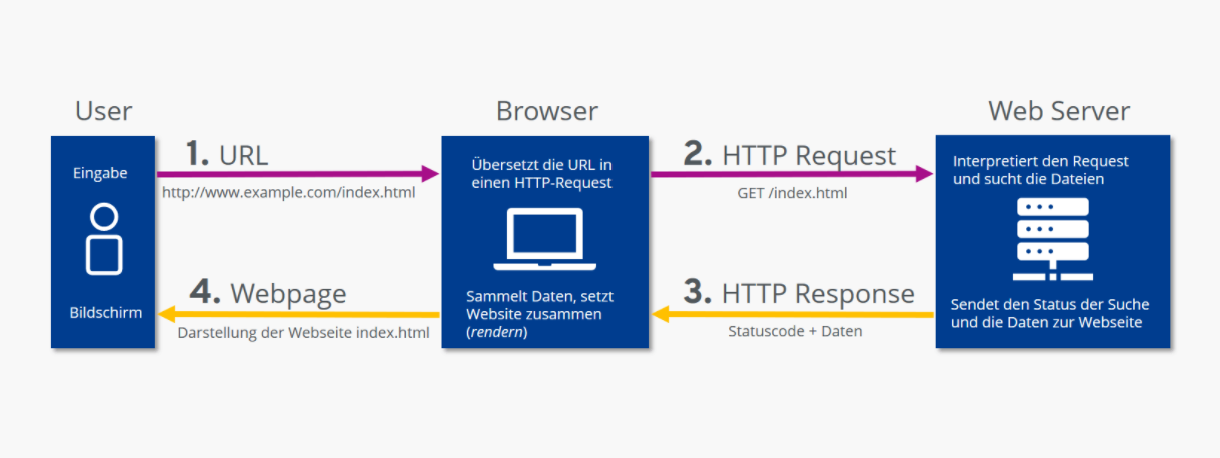
\includegraphics[width=10cm]{http.png}
\end{figure}
\\
\textbf{FTP/SFTP}\\
Das Protokoll ist dafür entwickelt worden, um mit Befehlen Downloads und Uploads imm Zusammenhang mit dem entsprechenden Server durchzuführen. So kann man Dateien von dem eigenen Gerät (PC, Smartphone usw.) auf einen Server übertragen auch und umgekehrt. Per FTP können Dateien auch vom Server auf das Gerät heruntergeladen werden.
Das File Transfer Protocol findet Anwendung beim Erstellen von Websites, weil mit dem FTP-Zugang können HTML-Dateien auf den Server übertragen werden. Außerdem können Betreiber von Websites Mediendateien für Besucher der Homepage bereitstellen.
SSH File Transfer Protocol (SFTP) hingegen verwendet die Secure Shell für die sichere Übertragung von Dateien. Auch hierbei ist die Verbindung verschlüsselt.
\begin{figure}[h]
    \centering
    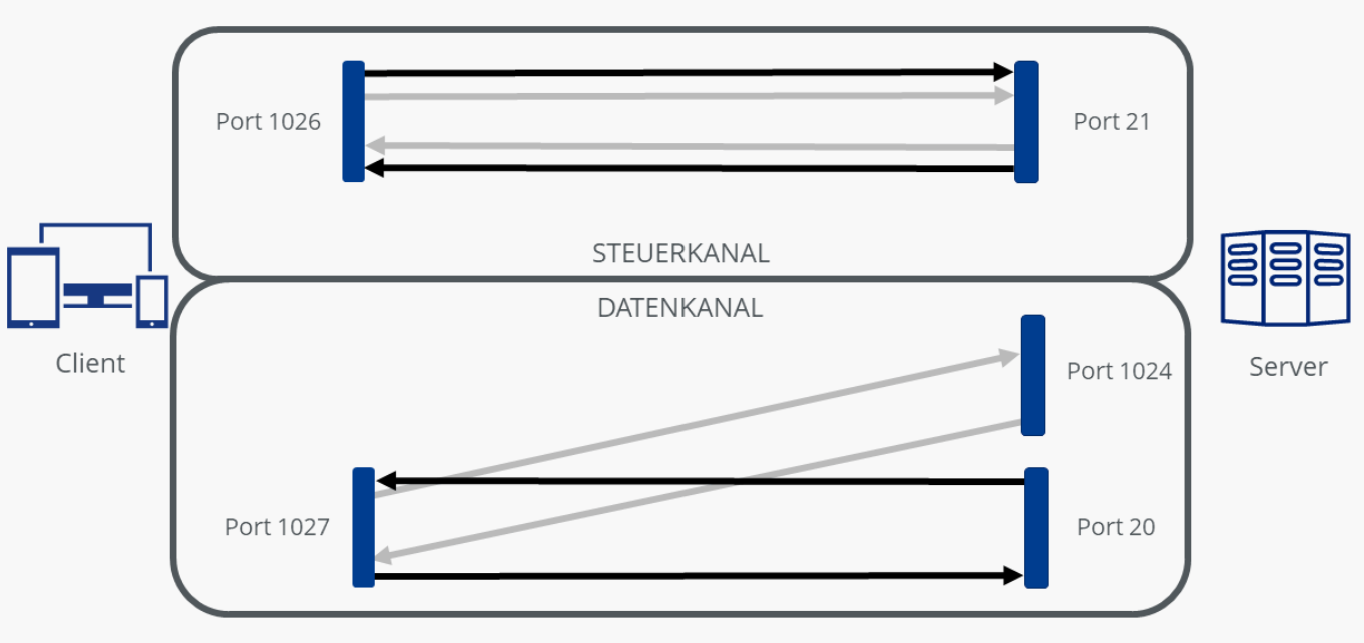
\includegraphics[width=10cm]{ftp.png}
\end{figure}
\newpage
\noindent
\begin{description}
    \item[TCP/IP-Modell] ~\par
    \begin{itemize}
        \item Netzzugangsschicht
        \begin{itemize}
            \item{Die Netzzugangsschicht ist zuständig, für die Verknüpfung von verschiedenen Subnetzen und verbindet so zum Beispiel das heimische WLAN per Router mit dem Internet.}
        \end{itemize}
        \item Internetschicht
        \begin{itemize}
            \item{Das Internetprotokoll ist an diese Schicht gerichtet, weil dadurch die Daten an das richtige Ziel gesendet werden soll.  Über die IP-Adresse werden die Datenpakete durch das Netzwerk geroutet.}
        \end{itemize}
        \item Transportschicht
        \begin{itemize}
            \item{In diese Schicht kommt das Protkoll TCP zum Vorschein.  Das Protokoll ermöglicht die Ende-zu-Ende-Kommunikation, ist also verantwortlich für die Verbindung zwischen zwei Geräten. Neben TCP gehört auch UDP in diese Ebene.}
        \end{itemize}
        \item Anwendungsschicht
        \begin{itemize}
            \item{Die Kommunikation der Programme über das Netzwerk wird in der obersten Schicht geregelt. Maßgeblich sind hier z.B. HTTP und FTP. Aber auch die E-Mail-Kommunikation mittels POP, SMTP funktioniert auf dieser Ebene.}
        \end{itemize}
    \end{itemize} 
\end{description}
\begin{figure}[h]
    \centering
    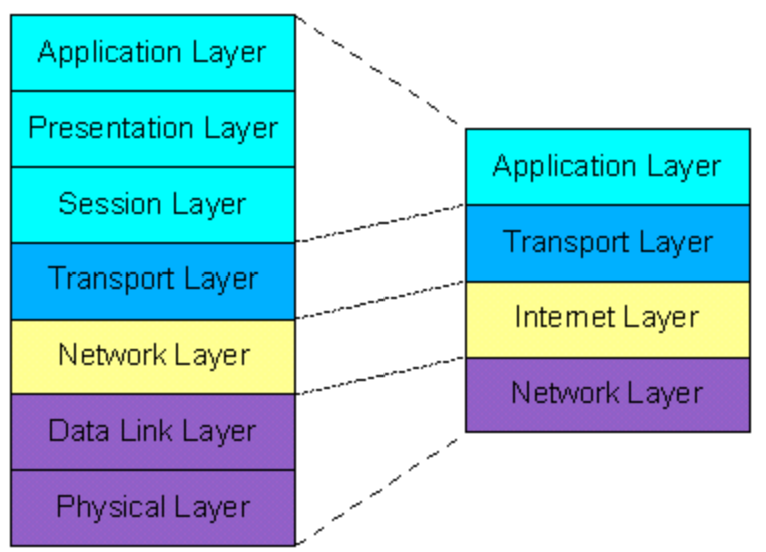
\includegraphics[width=10cm]{ositcpip.png}
\end{figure}
\cite{tcpip}
\newpage
\noindent
\section{Implementierung}
In diesem Kapitel geht es grundsätzlich um die technische Realisierung der
Aufgabenstellung. Im folgendem Abschnitt wird auch der Aufbau des Projekts
beschrieben. Außerdem enthält dieses Kapitel auch die Dokumentation
des Source Codes und wichtige Informationen bezgüglich Bibliotheken, die
im Projekt verwendet wurden.
\subsection{Projektstruktur}
Das Projekt wird ein drei wesentliche Verzeichnise eingeteilt, nämlich declaration, documentation und source. In dem Verzeichnis declaration sind alle Unterlagen abgelegt, die als Projektinput dient. In diesen Dokumenten sind die genauen Vorgaben des jeweiligen Projekts festgehalten. Im Ordner documenation sind alle Dateien der theoretischen Ausarbeitung des Themas und der Realisierung des Projekt abgespeichert, wohingegen im source Verzeichnis alle Datein der technischen Realisierung abgesichert werden.
Im Verzeichnis source gibt es drei Unterverzeichnisse dem build Ordner, indem alle generierten Datein abgespeichert werden, der include Ordern, indem alle Header-Datein abgelegt werden und der src Folger, in diesem sind die main.cpp Dateien und die dazugehörigen .cpp Dateien des .h Dateien. Das Projekt wird in Module eingeteilt. Das heißt die Klassendefinition,
Konstruktoren und Methodenprototypen von Client, SlaveServer und MasterServer stehen in der jeweiligen h-Datei.
Die Methodendefinitionen, der dazugehörigen Klasse, wurden in der dazugehörigen cpp-Datei kodiert.
Zusätzlichen Funktionen die für die Umsetzung des Projekts dringend notwendig
waren, wurden in dem Modul utils declariert und definiert. 
Der Compiler generiert drei auszuführende Programm, dem Client, dem SlaveServer und dem MaterServer. Welche Zielsetzungen die einzelnen Programme haben wird im jeweiligen Verzeichnis beschrieben.
Da einige Source Code Abschnitte nicht verständlich und nachfollziebar sind, wurden
alle Variablen, Funktionen, Klassen, Methoden und sonstiges gut dokumentiert.
\newpage
Im unterem Verzeichnisbaum wird die Struktur des Projektes abgebildet
\\
\dirtree{%
.1 declaration\DTcomment{enthält alle Dateien die für die Umsetzung}.
.2 {issues.pdf}.
.2 {projects.pdf}.
.1 documentation\DTcomment{enthält alle Dateien der theoretiscenh Ausarbeitung}.
.2 {MapReduce\_System\_Dokumentation.pdf}.
.2 {MapReduce\_System\_Dokumentation.tex}.
.2 {literatur.bib}.
.1 source\DTcomment{enthält alle Dateien der praktischen Ausarbeitung}.
.2 build\DTcomment{darin befinden sich alle automatisch generiert Datein}.
.2 include\DTcomment{darin befinden sich alle h-Dateien}.
.3 {client.h}.
.3 {slaveserver.h}.
.3 {masterserver.h}.
.3 {utils.h}.
.2 src\DTcomment{darin befinden sich alle cpp-Dateien}.
.3 {client}.
.4 {client.cpp}.
.4 {main.cpp}.
.4 {clientfile.txt}.
.3 {masterserver}.
.4 {masterserver.cpp}.
.4 {main.cpp}.
.3 {slaveserver}.
.4 {slaveserver.cpp}.
.4 {main.cpp}.
.4 {data.json}.
.3 {utils.cpp}.
}
\newpage
\noindent
\subsection{UML Klassendiagramm}
\:
\:
\begin{figure}[h]
    \centering
    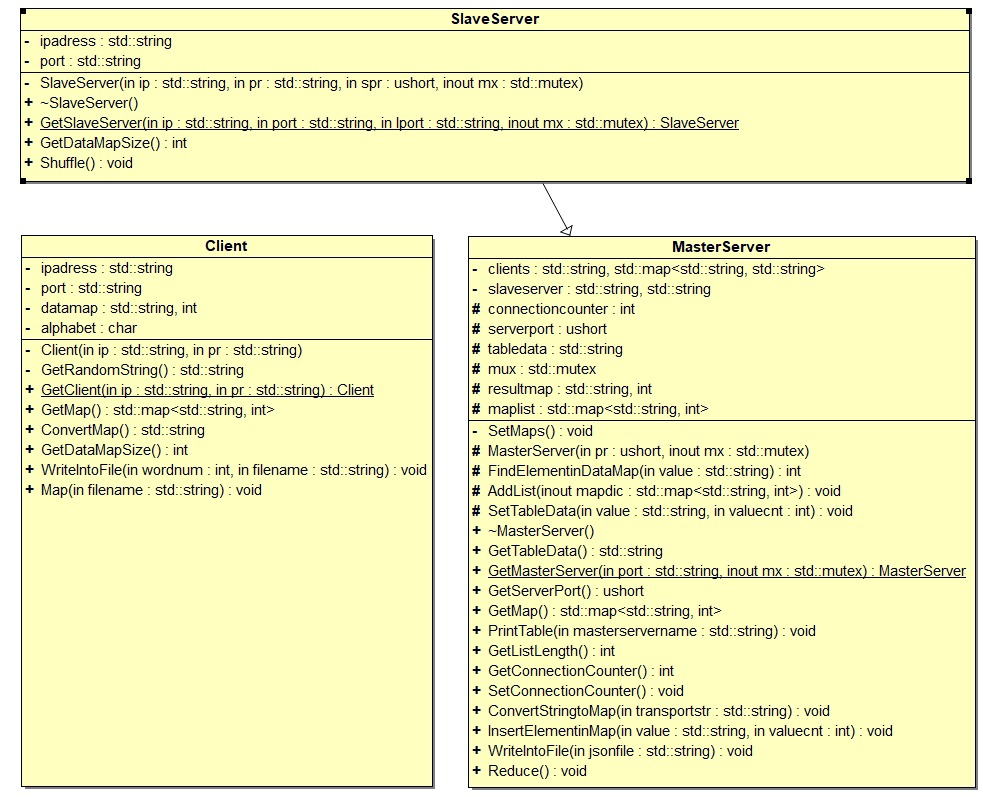
\includegraphics[width=12cm, height=12cm]{uml.jpeg}
\end{figure}
\newpage
\subsection{Client}
\textbf{Modulbeschreibung}\\
Die Komponente Client ist eine ausführbare Datei und bildet den Input für die Datenverarbeitung des MapReduce-Systems. Wenn das Programm vom Benutzer gestartet wird, wird eine Verbindung zum jeweiligen Server aufgebaut. Wenn diese erfolgt, wird eine bestimmte Anzahl von Strings, 
die der Benutzer beim Aufruf mitübergibt, generiert und in eine Datei geschrieben. In der nächsten Phase durchforstet das Programm, die Datei zeilenweise durch und speichert die Datensätze in einer Art Dictionary ab(Key:Value). Der zufällig generierte String entspricht im Dictionary dem Key und der Value die Anzahl des Strings wie oft dieser in der Datei vorkommt.
Diesen Part wird im MapReduce-System als Map Funktion bezeichnet. Zum Schluss wenn alle Daten im Dictionary abgespeichert sind, wird dieses in einem
String konvertiert, um diesen daraufhin an dem Server zu übertragen. Bei der Umwandlung des Dictionarys, werden den Key-Werten und Value-Werten Trennsymbole angehängt, sodass der Slaveserver die Zeichenkette aufteilen und weiters in ein Dictionary zurück umkonvertieren kann.\\\\
\textbf{Kommandozeilenparameter}\\
\begin{minted}{cpp}
MapReduceSystem_Client
Usage: ./client [OPTIONS]

Options:
  -h,--help                   Print this help message and exit
  -n,--n TEXT REQUIRED        name for the client
  -i,--i TEXT                 ipadress for the client
  -p,--p TEXT REQUIRED        port to connect to
  -f,--f TEXT:FILE            filepath of the file

\end{minted}
\newpage
\textbf{Klassenaufbau}\\

\subsection{SlaveServer}
\textbf{Modulbeschreibung}\\
Diese Komponente bildete die Schnittstelle zwischen den Clients und dem Masterserver. Der SlaveServer hört auf einen Port ab und empfängt, jene Daten die ihm der Client sendet. Die Übetragungsdaten wird in Form von einem String übertragen, wobei die 
einzelnen Werte durch ein ; getrennt werden. Wenn der Slaverserver von 2 unterschieldichen Clients Daten bekommen hat, werden die Strings zurück in eine Map konvertiert und in einer Map-List abgespeichert. Wenn sich zwei Maps in dieser Liste befinden, wird zu jedem Paar(also wenn immer 2 Maps in der Liste gespeichert sind)
ein Thread gestartet. In jedem Thread werden die einzelnen Werte eine Map vergliechen und verkleinert, d.h Durchführung der Shuffle Phase. Die resultierenden Daten werden dann in der Map datamap abgespeichert. Da alle erzeugten Threads ihre Daten in der datamap abspeichern, werden redundante Daten erzeugt. Diese müssen schlussendlich auch komprimiert werden. Am Ende dieser Phase werden alle Daten in der resultmap abspeichert. 
Auf Grund der parallele Abarbeitung der Daten bietet, dieses System eine hohe effizienz. Wie im Modul Client wird die Map am Ende zu einem Übertragungsstring umgewandlet und dem MasterServer versendet.
\textbf{Kommandozeilenparameter}\\
\begin{minted}{cpp}
MapReduceSystem_SlaverServer
Usage: ./slaveserver [OPTIONS]

Options:
  -h,--help                   Print this help message and exit
  -n,--n TEXT REQUIRED        name for the slaveserver
  -i,--i TEXT                 ipadress for the server
  -p,--p TEXT REQUIRED        port to connect to
  -s,--s TEXT REQUIRED        serverport
  -c,--c INT                  the maximum of clients

\end{minted}
\textbf{Klassenaufbau}\\
\subsection{MasterServer}
\textbf{Modulbeschreibung}\\
\textbf{Kommandozeilenparameter}\\ 
\begin{minted}{cpp}
MapReduceSystem_MasterServer
Usage: ./masterserver [OPTIONS]

Options:
  -h,--help                   Print this help message and exit
  -n,--n TEXT REQUIRED        name for the masterserver
  -p,--p TEXT REQUIRED        serverport
  -c,--c INT                  the maximum of slaveserver
  -j,--j TEXT:FILE            write reduced data in json-file
  -t,--t                      print a table about the reduced data

\end{minted}
\textbf{Klassenaufbau}\\
\subsection{utils}
\textbf{Funktionen}\\
\subsection{Konsolenausgabe}
\newpage
\noindent
\subsection{Verwendete Bibliotheken}
\subsubsection{asio}
Asio ist eine plattformübergreifende C++-Bibliothek für Netzwerk- und Low-Level-I/O-Programmierung, die Entwicklern ein konsistentes asynchrones Modell mit einem modernen C++-Ansatz bietet.
Asio bietet die grundlegenden Bausteine für C++-Netzwerke, Gleichzeitigkeit und andere Arten von Eingabe/Ausgabe
Asio wird in allen Arten von Anwendungen eingesetzt, von Telefon-Apps bis hin zu den schnellsten Aktienmärkten der Welt.\\\\
Die meisten Programme interagieren auf irgendeine Weise mit der Außenwelt, sei es über eine Datei, ein Netzwerk, ein serielles Kabel oder die Konsole. Manchmal, wie z. B. bei Netzwerken, können einzelne E/A-Operationen sehr lange dauern, bis sie abgeschlossen sind. Dies stellt besondere Herausforderungen an die Anwendungsentwicklung.
Asio stellt die Werkzeuge zur Verfügung, um diese langwierigen Operationen zu verwalten, ohne dass die Programme Gleichzeitigkeitsmodelle auf Basis von Threads und explizitem Sperren verwenden müssen.
Die Asio-Bibliothek ist für Programmierer gedacht, die C++ für die Systemprogrammierung verwenden, bei der häufig der Zugriff auf Betriebssystemfunktionen wie z. B. Netzwerke erforderlich ist. Obwohl sich Asio anfangs hauptsächlich auf Netzwerke konzentrierte, wurden seine Konzepte der asynchronen I/O auf andere Betriebssystemressourcen wie serielle Schnittstellen, Dateideskriptoren usw. erweitert.
\cite{asio}
\begin{description}
    \item[Im Besonderen verfolgt Asio folgenden Ziele:] ~\par
    \begin{itemize}
        \item Portability
        \begin{itemize}
            \item{Die Bibliothek sollte eine Reihe gängiger Betriebssysteme unterstützen und ein konsistentes Verhalten über diese Betriebssysteme hinweg bieten.}
        \end{itemize}
        \item Scalability
        \begin{itemize}
            \item{Die Bibliothek sollte die Entwicklung von Netzwerkanwendungen erleichtern, die auf Tausende von gleichzeitigen Verbindungen skalieren. Die Implementierung der Bibliothek für jedes Betriebssystem sollte den Mechanismus verwenden, der diese Skalierbarkeit am besten ermöglicht.}
        \end{itemize}
        \item Efficiency
        \begin{itemize}
            \item{Die Bibliothek sollte Techniken wie Scatter-Gather-I/O unterstützen und es Programmen ermöglichen, das Kopieren von Daten zu minimieren.}
        \end{itemize}
        \item Model concepts from established APIs, such as BSD sockets
        \begin{itemize}
            \item{Die BSD-Socket-API ist weithin implementiert und verstanden und wird in viel Literatur behandelt. Andere Programmiersprachen verwenden oft eine ähnliche Schnittstelle für Netzwerk-APIs. Soweit dies sinnvoll ist, sollte Asio die bestehende Praxis nutzen.}
        \end{itemize}
        \item Ease of use
        \begin{itemize}
            \item{Die Bibliothek sollte eine niedrigere Einstiegshürde für neue Benutzer bieten, indem sie eher einen Toolkit- als einen Framework-Ansatz verfolgt. Das heißt, sie sollte versuchen, den zeitlichen Aufwand im Vorfeld auf das Erlernen einiger grundlegender Regeln und Richtlinien zu minimieren. Danach sollte ein Bibliotheksbenutzer nur noch die spezifischen Funktionen verstehen müssen, die verwendet werden.}
        \end{itemize}
        \item Basis for further abstraction
        \begin{itemize}
            \item{Die Bibliothek sollte die Entwicklung anderer Bibliotheken ermöglichen, die eine höhere Abstraktionsebene bieten. Zum Beispiel Implementierungen von häufig verwendeten Protokollen wie HTTP.}
        \end{itemize}

    \end{itemize} 
\end{description}
\subsubsection{CLI11}
CLI11 bietet alle Funktionen, die man von einem leistungsstarken Befehlszeilenparser erwartet, mit einer schönen, minimalen Syntax und ohne 
Abhängigkeiten über C++11 hinaus. Es ist eine header-only, um die Einbindung in Projekte zu 
vereinfachen. CLI11 ist einfach für kleine Projekte zu verwenden, aber leistungsstark genug für komplexe Befehlszeilenprojekte und kann für Frameworks angepasst werden. \\\\
Die Bibliothek wird mit Travis-, AppVeyor-, Azure- und GitHub-Aktionen getestet und vom GooFit-GPU-Anpassungsframework verwendet. 
Es wurde von plumbum.cli für Python inspiriert. CLI11 bietet eine benutzerfreundliche Einführung in diese README-Datei, ein ausführlicheres Tutorial-GitBook, sowie eine von Travis generierte API-Dokumentation. 
Weitere Informationen zu aktuellen und früheren Versionen findet man im Changelog oder in den GitHub-Versionen.
\cite{cli11}
\subsubsection{spdlog}
spdlog ist eine sehr effiziente headeronly C++ Protokollierungsbibliothek. Sie bietet auch ebenfalls eine Python-ähnliche Formatierungs-API unter Verwendung der mitgelieferten fmt lib.
spdlog verfolgt den Ansatz "include what you need". Der Source Code sollte die Funktionen enthalten, die tatsächlich benötigt werden.\\\\
Den Programmierer wird eine funktionsreiche Formatierung mit der hervorragenden fmt-Bibliothek geboten.
Im Projekt wird die Libary verwendet, damit die Logging Informationen in der Kommandozeile ausgegeben werden kann. Zusätzlich ist es auch möglich,
die Logging Daten nicht nur auszugeben, sonder auch direkt in einem Log-File zu schreiben.
\cite{spdlog}
\subsubsection{json}
In Sprachen wie Python fühlt sich JSON wie ein erstklassiger Datentyp an.
Die Entwickler haben die ganze Operator-Magie des modernen C++ verwendet, um das gleiche Gefühl in einem c++ Projekt zu erzielen. 
Der gesamter Code besteht aus einer einzelnen Header-Datei json.hpp. Keine Bibliothek, kein Teilprojekt, keine Abhängigkeiten, kein komplexes Build-System. 
Die Klasse ist in Vanilla C++ 11geschrieben. \\\\
Alles in allem ist keine Anpassung der Compiler-Flags oder Projekteinstellungen erforderlich.
Jedes JSON-Objekt hat einen Overhead und ein Aufzählungselement. Die Standardverallgemeinerung verwendet die folgenden C++-Datentypen: std::string für Zeichenfolgen, int64\_t, uint64\_t oder double für Zahlen, std::map für Objekte, std::vector für Arrays und bool für Boolesche Werte. 
json.hpp ist die einzige erforderliche Datei in single\_include/nlohmann, jedoch muss sie im Projekt mit eingebunden werden. \\
Die Libary wurde in diesem Projekt verwendet, um die zusammengefassten Daten des Master-Server abzuspeichern.
\cite{json}
\subsubsection{rang}
rang only hängt von der C++ Standardbibliothek, dem Systemheader unist d.h unter Unix und den Systemheadern windows.h und io.h auf Windows\-basierten Systemen ab. Mit anderen Worten, man benötigt keine Abhängigkeiten von Drittanbietern. Diese Standardbibliothek ermöglich es den
Output der Console zu formatieren. Dabei kann die Schriftart, Farbe und sonstige Eigenschaften bezüglich der Consolenausgabe konfigurieren.
\cite{rang}
\newpage
\noindent
\subsubsection{tabulat}
tabulate ist eine reine headeronly-Bibliothek. 
Man legt eine Objekt Table an und kann mittel Table.add\_rows neue Zeilen in der Tabelle hinzufügen.
Die Tabelle kann mittels Table.format() formatiert werden, das ein Format-Objekt zurückgibt. 
Es können damit die Eigenschaften der Tabelle formatiert werden, z. B. Rahmen, Schriftstile, Farben usw.
Auf Zeilen in der Tabelle greift man mitTabelle [row\_index] zu. Dies gibt ein Zeilenobjekt zurück, für das man Row.format() auf ähnliche Weise aufrufen kann, um die Eigenschaften aller Zellen in dieser Zeile zu formatierne.\\
Die Bibliothek wurde verwendet, sodass am Ende des Programmes eine übersichtliche Tabelle ausgegeben werden kann, wie viele Daten in Struktur gebracht wurden.
beinhaltet.
\cite{tabulate}
\section{Anwendungsfälle}

\section{Schlusswort}
\newpage
\printbibliography
\end{document}
